%!TEX root = Thesis.tex

\chapter{Lexicon acquisition and annotation}
\label{chap:lexiconAcquisition}

For small language fragments the lexicon can simply be ``handwritten'', as demonstrated in the previous chapter.  However this is obviously not an sane option when the grammar is to accept a large vocabulary and a wide range of sentence structures.

In order to use the presented model on a actual data, the acquisition of a wide covering lexicon is crucial. Initially considerable effort was made to \emph{try} to build a CCG lexicon from a \emph{POS-tagged corpus} (part-of-speech-tagged corpus). A POS-tagged corpus is simply a corpus where each token is tagged with a POS-tag, e.g.\ noun, verb, etc. There is no deep structure in such a corpus as opposed to a \emph{treebank}. This approach turned up to have extensive issues as a result of this lack of structure, some of which are detailed in Appendix~\ref{chap:brownCorpus} which succinctly describes the process of the attempt.

There exists some wide covering CCG lexicons, most notable \emph{CCGbank}, compiled by \citeauthor{ccgBank} \shortcite{ccgBank} by techniques presented by \cite{juliaThesis}. It is essentially a translating of almost the entire Penn Treebank \cite{pennTreebank}, which contains over 4.5 million tokens, and where each sentence structure has been analyzed in full and annotated. The result is a highly covering lexicon, with some entries having assigned over 100 different lexical categories. Clearly such lexicons only constitutes half of the previous defined $\mathcal{L}_\mathrm{CCG}$ map, i.e.\ only the lexical categories, $\Gamma$. The problem of obtaining a full lexicon, that also yields semantics expressions, is addressed in the next section. It is also worth mentioning that since \citeauthor{baldridgeThesis}'s \shortcite{baldridgeThesis} work on modalities only slightly predates \citeauthor{juliaThesis}'s \shortcite{juliaThesis} work on CCGBank, the CCGBank does not incorporate modalities\footnote{There does exists another project, OpenCCG, started by \citeauthor{baldridgeThesis}, which actually does incorporate modalities, but it has little documentation and was therefore not valued mature enough.}. However more unfortunately is that CCGBank is not free to use, mainly due to license restrictions on the Penn Treebank.% It has not been possible to fund a license.

What might not be as obvious is that besides obtaining a wide-covering lexicon, $\mathcal{L}_\mathrm{CCG}$, a even harder problem is for some text $T$ to select the \emph{right} tagging from $\mathcal{L}_\mathrm{CCG}(w)$ for each token $w \in T$. \citeauthor{ccgBank} \shortcite{ccgBank} calculate that the expected number of lexical categories per token is 19.2 for the CCGBank. This mean that a exhaustive search of even a short sentence (seven tokens) is expected to consider over 960 million ($19.2^7 \approx 961.852.772$) possible taggings. This is clearly not a feasible approach, even if the parsing can explore all possible deductions in polynomial time of the number of possible taggings. %, e.g.\ \cite{shiftReduceChart}. 
The number of lexical categories assigned to each token needs to be reduced, however simple reductions as just assigning the most frequent category  observed in some training set (for instance CCGBank) for each token is not a solution. This would fail to accept a large amount of valid sentences, simply because it is missing the correct categories. 

\section{Maximum entropy tagging}
Clearly a solution need to base the reduction on the setting of the token, i.e.\ in which \emph{context} the token appears. \citeauthor{suppertagging} \shortcite{suppertagging} presents a \emph{maximum entropy model} that estimate the probability that a token is to be assigned a particular category, given the \emph{features} of the local context, e.g.\ the POS-tag of the current and adjacent tokens, etc. This is used to select a subset of possible categories for a token, by selecting categories with a probability within a factor of the category with highest probability. \citeauthor{suppertagging} shows that the average number of lexical categories per token can be reduced to 3.8 while the parser still recognize 98.4\% of unseen data. \citeauthor{candc} \shortcite{candc} presents a complete parser, which utilizes this tagging model, and a series of (log-linear) models to speed-up the actual deduction (i.e.\ the parsing) once the tagging model has assigned a set of categories to each token. What maybe even more interesting is that models trained on the full CCGBank, along with toolchain to use them (called the C\&C tools), can be licensed freely for education or research purposes. For this reason it was chosen to use these models and tools.

Furthermore, even though the models neither incorporates modalities, since they are trained on the CCGBank, the deduction models solve many of these problems, since a more plausible deduction (i.e.\ a deduction seen more frequent in the CCGBank) always will suppress other less plausible deductions. Special care are taken about coordination, so neither here seems the lack of modalities to yield significant issues.


\clearpage

\section{Annotating the lexicon}
The output from the C\&C toolchain can be printed in various formats, including Prolog, which was considered the closest to the presented model, as it, given some set of tokens, $w_1, \ldots, w_n$, simply returns a lexicon and a deduction. A illustrative output for the tokens ``the service was great'' is given in Figure~\ref{fig:candcOutput}. In Chapter~\ref{chap:implementation} more details on the actual format and the processing of it is given.
\begin{figure}[ht]
	\begin{minipage}[b]{0.6\linewidth}
	\center
	\begin{align*}
\alpha_1 &\equiv \mathbf{the} : \mathrm{the}_{\textsc{dt}} \models \cat{NP}_\mathrm{nb} / \cat{N} \\
\alpha_2 &\equiv \mathbf{service} : \mathrm{service}_{\textsc{nn}} \models \cat{N} \\
\alpha_3 &\equiv \mathbf{was} : \mathrm{be}_{\textsc{vbd}} \models (\cat{S}_\mathrm{dcl} \bsl \cat{NP}) / (\cat{S}_\mathrm{adj} \bsl \cat{NP}) \\
\alpha_4 &\equiv \mathbf{great} : \mathrm{great}_{\textsc{jj}} \models \cat{S}_\mathrm{adj} \bsl \cat{NP}
	\end{align*}
	(a) Lexicon
	\end{minipage}
	\hfill
	\begin{minipage}[b]{0.4\linewidth}
	\center
	$$
	  \inference[<]{  
	    \inference[>]{
	      \alpha_1 \;
	      \alpha_2
	    }{
	      \cat{NP}_\mathrm{nb}
	    }
	    \inference[>]{
	      \alpha_3 \;
	      \alpha_4
	    }{
	      \cat{S}_\mathrm{dcl} \bsl \cat{NP}
	    }
	  }{
	    \cat{S}_\mathrm{dcl}
	  }
	$$
	(b) Deduction
	\end{minipage}
	\caption{Illustration of output from the C\&C toolchain.}
	\label{fig:candcOutput}
\end{figure}

Clearly, deductions in the style previously presented is trivially obtained by substituting the axioms placeholders with the lexicon entries associated. The C\&C toolchain also has a build-in morphological analyzer which allow the lexicon to provide the \emph{lemma} of the tokens. This will be convenient later. Furthermore the lexicon also provide the POS-tag of the token which also will prove itself useful.

\clearpage

\section{Calculating sentiment values}
In order to reason about the polarity of the selected subject in the review text, a understanding of the domain of the review is needed.  For this purpose the concept of \emph{semantic networks} is introduced. Formally it is defined follows:
\begin{definition}
a semantic network is a quadruple $(L,S,R,M)$ where:\\[-2em]
  \begin{itemize} %[labelindent=2em,labelwidth=0em,itemindent=0em,leftmargin=2em]
    \item $L$ is the set of lexical units recognized by the network.
    \item $S$ is the set of \emph{semantic concepts} in the network.
    \item $R$ is a set of binary relations on $S$ where the relation $r \in R$ describes links\\ between semantic concepts, i.e.\ $r \subset S \times S$. 
    \item $M$ is a mapping from lexical units to a set of semantic entities that the lexical\\ unit can entail, i.e.\ $M: L \to \mathcal{P}(S)$.
  \end{itemize}
  \label{def:SemanticNetwork}
\end{definition}

Notice that $S$ and $R$ constitutes a set of graphs, i.e.\ for each relation $r \in R$ the graph~$(S,r)$. The graph is undirected if $r$ is \emph{symmetric}, and directed if $r$ is \emph{asymmetric}.

\begin{figure}[ht]
  \center
  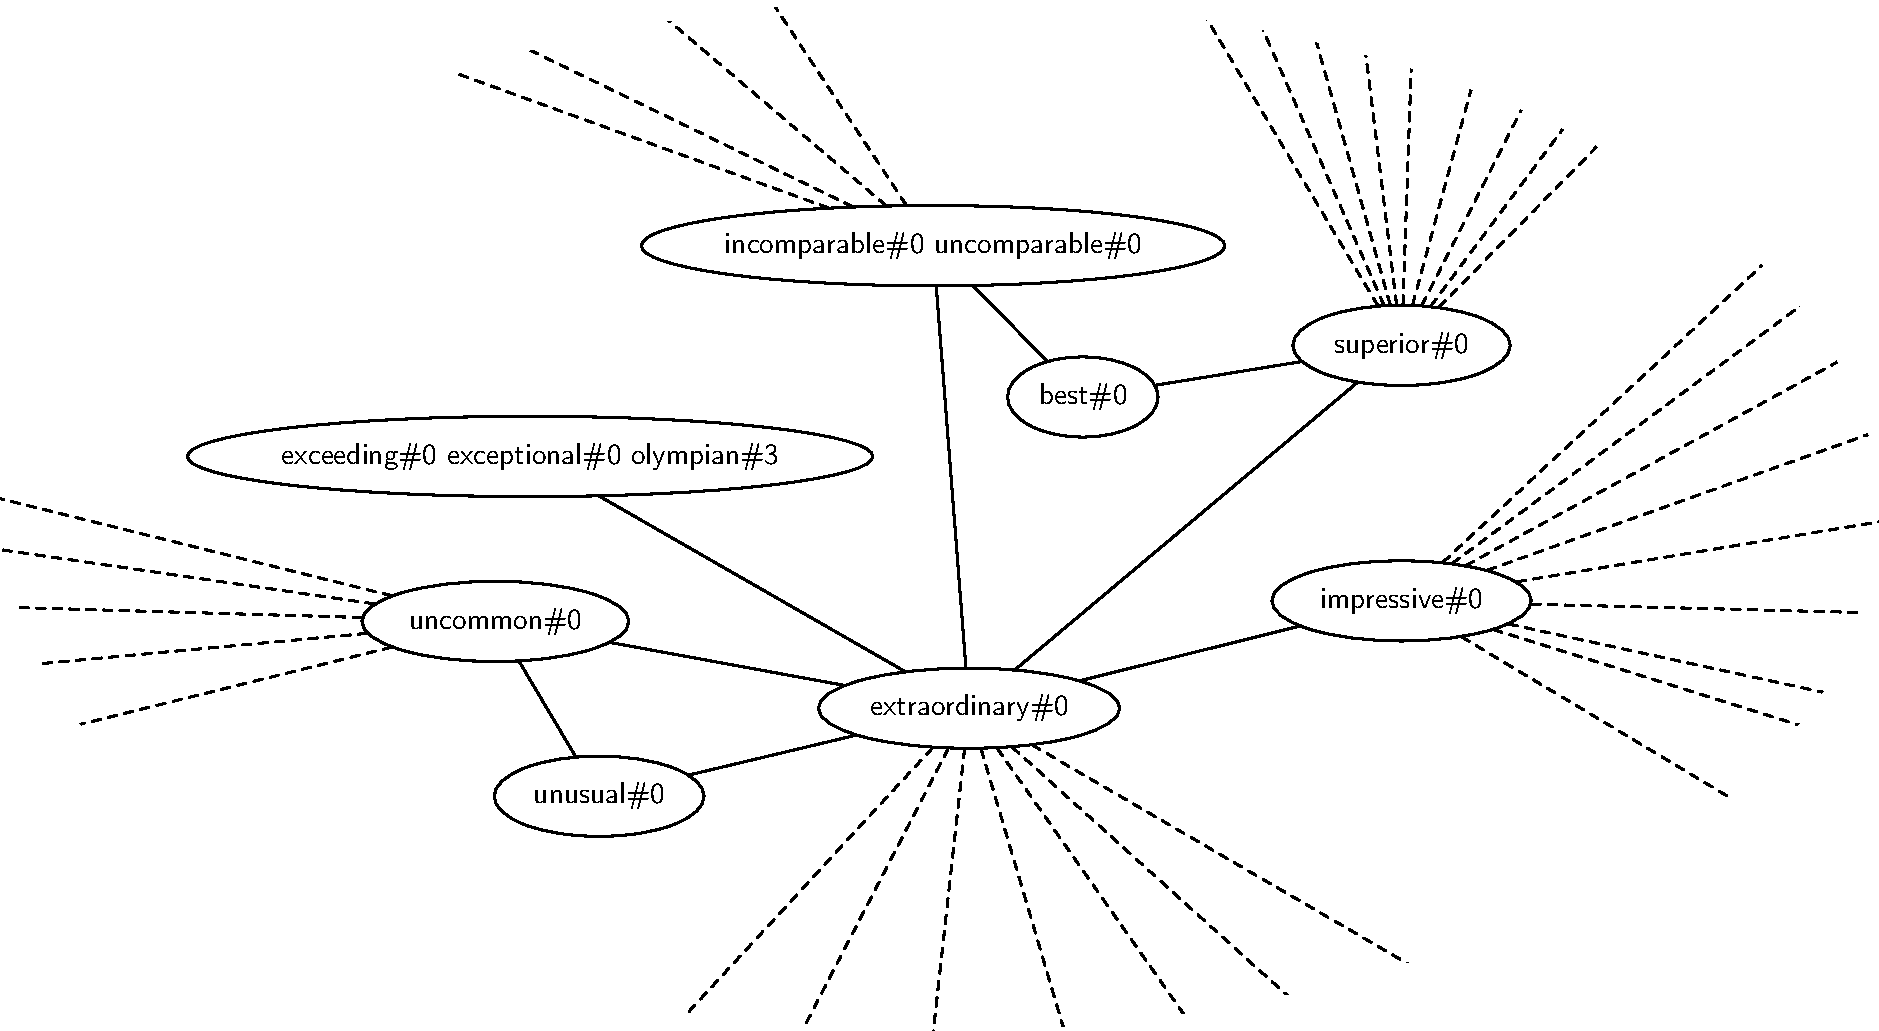
\includegraphics[scale=.4]{Figures/Exceptional}
\end{figure}

\cite[p. 453-456, 468, 471]{ai}

An illustrative example of such a graph, denoting a relation in a tiny semantic network of adjective concepts is given in figure X. The relation depictured . 
transitivity...


We have no way of detecting different semantic ambiguity, since we have no knowledge bade ... therefore we shall restrict our-self to 